\documentclass[11pt]{amsart}

\usepackage[letterpaper,left=125pt,right=125pt]{geometry}

% ^^^^^^^^^^^^^^^^^^^^^^^^^^^^^^^^^^^^^^^^^^^^^^^^^^^^^^^^^^^^^^^^^
% DO NOT change anything above this line! 
% (We need standard margins and type size.)
% In particular, don't include your own "geometry" settings further down.



%%%%%%%%%%%%%%%%%%%%%%%%%%%%%%%%%%%%%%%%%%%%%
% The following part of the preamble sets up packages, theorems, and shortcuts; 
% you can edit it, but you won't need to change much.

%% Load Packages:

\usepackage[english]{babel}
\usepackage {amsmath}  % provides lots--- e.g. equations, matrices, definition by cases
\usepackage{amssymb}  % provides common mathematical symbols
\usepackage{amsfonts}
\usepackage{amsthm}     %provides \newtheorem, \theoremstyle, \begin{proof}...\end{proof}
\usepackage{graphicx}  % allows importation of graphics files

\usepackage[colorlinks,linkcolor=blue,citecolor=blue,urlcolor=blue]{hyperref} % typesets URLS and clickable cross-references and links
%\usepackage{hyperref} % if you don't want colored links, just use the simpler command


\usepackage[backend=bibtex]{biblatex} % bibliography support
\addbibresource{sample.bib} % CHANGE this to the name of your BibTeX database file (see instructions below)

%% Environments for theorems, etc.. 

% You can add your own theorem-like environments, see https://en.wikibooks.org/wiki/LaTeX/Theorems
% The basic format is \newtheorem{name}{display-text}[numbered-within] or \newtheorem{name}[numbered-like]{display-text}

\theoremstyle{theorem} % set the style for the following theorems

\newtheorem{thm}{Theorem}[section] %\newtheorem{name}{display-text}[numbered-within]

\newtheorem{lem}[thm]{Lemma} %\newtheorem{name}[numbered-like]{display-text}
\newtheorem{cor}[thm]{Corollary}
\newtheorem{prop}[thm]{Proposition}
\newtheorem{alg}[thm]{Algorithm}

\theoremstyle{definition}                  % switch to a different style
\newtheorem{defn}[thm]{Definition}
\newtheorem{conj}[thm]{Conjecture}


\theoremstyle{example}                       % another style
\newtheorem{prob}[thm]{Problem}


\theoremstyle{remark}                       % another style
\newtheorem{exmp}[thm]{Example}  % (note:the "example" style is not really good for long examples-- typesets them in italics!)
\newtheorem{rem}[thm]{Remark}
\newtheorem{claim}[thm]{Claim}  
\renewcommand{\theclaim}{}

%% If you use numbered equations in a long document, it is preferred to number
% as (x.y), where x is section number, y is equation number

\numberwithin{equation}{section}


%% Common typesetting for common mathematical objects

\newcommand{\R}{\mathbb{R}}
\newcommand{\Q}{\mathbb{Q}}
\newcommand{\N}{\mathbb{N}}
\newcommand{\Z}{\mathbb{Z}}
\DeclareMathOperator{\rank}{rank}
\DeclareMathOperator{\dimension}{dim}



%%%%%%%%%%%%%%%%%%%%%%%%%%%%%%%%%%%%%%
% BEGIN: You'll _need_ to edit everything below....


%  Your data for title, author, etc.

\title[Math Thesis Template]{Mathematics Thesis Template} % here, the command format is  \title[Abbreviated Title for Header]{Full Title}. But if your title is short, simply use \title{Full Title}
\thanks{This document is a senior thesis submitted to the Mathematics and Statistics Department of Haverford College in partial fulfillment of the requirements for a major in Mathematics.} % REQUIRED: don't change this line
\author{Your name here}
\date{2019-01-21} % don't forget to update the date!

\begin{document}

\begin{abstract} % REQUIRED (and needs to go before \maketitle)
This document is a template for the Math/Stats senior thesis. (An abstract is required.)
\end{abstract}

\maketitle % Actually typeset the title, author, etc.


\tableofcontents % OPTIONAL. See https://en.wikibooks.org/wiki/LaTeX/Document_Structure#Table_of_contents for more information.

%%-------------------------------------------------------------------------------------------------
%% CUT START: you can delete all of the following content, through "CUT STOP" below
\section{Introduction}

Use this template to typeset your thesis with standard margins and formatting. The text below has examples of various \LaTeX\ structures that will help you write a 
document that adheres to the professional standards of written mathematics. 
In the source file, all of the sample content is clearly delimited; once you have browsed the sample content, you can delete everything between the comments \texttt{CUT START} and \texttt{CUT STOP}---then you are ready to put in your own content.

Near the top of the source file, you will find the following comment

\smallskip
\begin{verbatim}
% ^^^^^^^^^^^^^^^^^^^^^^^^^^^^^^^^^^^^^^^^^^^^^^^^^^^^^^^^^^^^^^^^^
% DO NOT change anything above this line! 
% (We need standard margins and type size.)
% In particular, don't include your own "geometry" settings further down.
\end{verbatim}
\smallskip

You must heed these instructions; otherwise, your thesis will not satisfy the department's standards.


\section{Sectioning}

Think carefully about using sections and subsections in order to structure your document. 

\subsection{Section numbering}

In a long document, sections and subsections should generally be numbered (even though \LaTeX\ lets you suppress the numbering). 
This allows you to easily make cross-references; see Section~\ref{items}. % The tilde in the cross-reference is a non-breaking space, so that "Section" and the "1.2" don't wind up on different lines.
(Note: the cross-reference is colored because it is a clickable link. If you want to turn off the coloring, see the preamble of the \LaTeX\ source file.)

\subsection{Table of contents}
A benefit of carefully sectioning your document is that you can automatically generate a table of contents. A table of contents may not be appropriate for all theses; ask your advisor. 

\section{Clarity and cross-references} \label{items}

\subsection{Clarity}
In mathematical writing, it is good style to first name the objects that you'll be talking about (e.g.\ a group $G$ and a subgroup $H$ of $G$), and then to refer to them by name;  otherwise, you get stuck with ambiguous or overly complicated sentences. Thus, we prefer to write 
\begin{defn} \label{def:af1}
Let $G$ be a group. We say that $G$ is \emph{abelian-by-finite} if there is a normal subgroup $H\trianglelefteq G$ such that $H$ is abelian and the quotient $G/H$ is finite.
\end{defn}
rather than the more convoluted statement
\begin{defn}\label{def:af2}
A group is called \emph{abelian-by-finite} if it has a normal subgroup such this subgroup is abelian and the quotient of the group by the subgroup is finite. 
\end{defn}
\begin{rem}
Note that the defined terms in Definitions \ref{def:af1} and \ref{def:af2} are emphasized using the \verb+\emph+ command; this command chooses the right way to emphasize the text, given the style of the surrounding text.
\end{rem}

\subsection{Cross-references}
Similar to our preference for referring to mathematical objects by name, in a long document, we want to clearly refer to displayed items (equations, definitions, theorems, etc.).  So, make sure that all of the displayed items have numbers, then use the built \LaTeX\ cross-referencing commands.
For example, theorems, definitions, etc.\ are already set up in the template to be numbered by section:

\begin{thm} \label{thm:fermat}
If $p$ is prime, then for all $a\in \Z$, $a^p \equiv a \pmod{p}$. % note \pmod for "parentheses mod"; see https://vmuthu.livejournal.com/3054.html for other styles of "mod"
\end{thm}

\begin{defn}
A composite integer $b>1$ is a \emph{Fermat pseudoprime}, if for all $a\in \Z$, $a^b \equiv a \pmod{b}$.
\end{defn}

When you typeset a displayed equation, \verb+\begin{equation}...\end{equation}+ works like the basic commands  \verb+\[...\]+, but includes automatic numbering:

\begin{equation} \label{eqn:binary}
 \lim_{k \rightarrow \infty} \sum_{i=1}^{k} \left( \frac{1}{2}\right)^i = 1.
\end{equation}

Some writers will number every equation in the document, others will number only the ones that they know will be referred to later 
(e.g. equation \eqref{eqn:binary} is referred to now); 
check with your advisor for advice.\footnote{Note that the command \texttt{$\backslash$eqref} is used to produce the equation cross-reference; it produces equation-specific typesetting, i.e.\ parentheses.}

Note that sometimes important theorems, like Theorem~\ref{thm:fermat}, have names, or are given names in a document. Here's how to typeset a name for a theorem-like item:

\begin{thm}[Fermat's Little Theorem]\label{thm:flt}
See Theorem~\ref{thm:fermat}
\end{thm}

If the displayed item has a name, we can refer to it by name, but we still might need to specify the number (Theorem~\ref{thm:flt})  or at least the section number (Section~\ref{items}) to help the reader who wants to look it up.

We can also name equations, overriding the automatic numbering: 
\begin{equation}
\sum_{0 \leq k \leq n-1} {{n-1}\choose{k}} n^{n-1-k} (k+1)! = n^n \tag{Key Eq.}.
\end{equation}

\begin{rem} \label{rmk:rmk}
Sometimes, you will find that you want to refer to a specific idea or bit of prose that appears earlier in your body text; in this case, consider turning the text into a Remark (e.g.\ see Remark~\ref{rmk:rmk}) and then referring to it via a cross-reference. 
Similarly, if you find yourself referring to an example that was detailed in a paragraph, consider turning that paragraph into a numbered Example.
\end{rem}
\section{Some good typesetting practices}

If you need to typeset something complicated, chances are you are not the only one. Don't reinvent the wheel! 
Search online for techniques and packages  that let you write the \emph{structure} of what you want without fussing too much with the typesetting. 
Good sources are the \href{https://en.wikibooks.org/wiki/LaTeX}{LaTeX Wikibook} \cite{wikibook} for general advice, and the \href{https://tex.stackexchange.com/}{TeX-LaTeX Stack Exchange} for more advanced issues. 

Below are some examples. 

\subsection{Quotation marks}
The correct way to typeset quotation marks in \LaTeX\ is not obvious!
\begin{quotation}
LaTeX treats left and right quotes as different entities. For single quotes, a grave accent, ` (on American keyboards, this symbol is found on the tilde key; adjacent to the number 1 key on most keyboards) gives a left quote mark, and an apostrophe, ' gives a right. For double quotes, simply double the symbols, and LaTeX will interpret them accordingly. \cite[Chap. ``LaTeX/Text Formatting'', \S 3]{wikibook}
\end{quotation}
In other words, it's ``Quoth the raven'', not "Quoth the raven".  See the \href{https://en.wikibooks.org/wiki/LaTeX/Text_Formatting#Quote-marks}{Quote Marks section} in the LaTeX Wikibook \cite{wikibook} for more information.

\subsection{Displayed math}
For displayed equations without numbering, use either \verb+\[..\]+ or \verb+\begin{equation*}...\end{equation*}+. 
%Other environments have similar non-numbered versions, like \verb+\begin{equation*}...\end{equation*}+,  
Double dollar signs (\verb+$$..$$+) are discouraged, since they are \TeX\ commands, not \LaTeX, and in rare
  cases they cause typesetting problems when they interact with other \LaTeX\ features.  See \cite [\S 1.6]{tabu}.

\subsection{Lists}
\begin{enumerate}
\item Use the built-in list environments. \label{item1}
\item If you follow the advice in item~\ref{item1}, then you can take advantage of cross-referencing for enumerated lists.
\begin{enumerate}
\item You can also nest lists---
\item let \LaTeX\ worry about the numbering
\item while you worry about 
\begin{itemize}
\item structure and
\item content.
\end{itemize}
\end{enumerate}


\end{enumerate}



\subsection{Piecewise definitions}
\begin{equation}
\vec{F}(x,y)=
	\begin{cases}
		 \frac{\langle -y,x\rangle}{x^2+y^2} & \text{if } x^2+y^2\neq 0\\
		\langle 0,0\rangle & \text{otherwise}
	\end{cases}
\end{equation}
%Maybe the fraction should be larger:
%\begin{equation}
%\vec{F}(x,y)=
%	\begin{cases}
%		 \displaystyle \frac{\langle -y,x\rangle}{x^2+y^2} & \text{if } x^2+y^2\neq 0\\
%		\langle 0,0\rangle & \text{otherwise}
%	\end{cases}
%\end{equation}
See the \href{https://en.wikibooks.org/wiki/LaTeX/Advanced_Mathematics#The_cases_environment}{the Cases section} of the LaTeX Wikibook \cite{wikibook} for more information.


\subsection{Automatic sizing of parentheses}
The following equation doesn't look  good, because the parentheses
are not the correct size: 

\begin{equation}
\lim_{x \rightarrow \infty} (1+\frac{\alpha}{x})^x = e^\alpha
\end{equation}

Below we get correctly sized parentheses using the commands
\verb,\left(, and \verb,\right), in place of regular
parentheses. (This technique also works for 
square brackets, braces, etc.)
\begin{equation}
\lim_{x \rightarrow \infty} \left(1+\frac{\alpha}{x}\right)^x = e^\alpha
\end{equation}

Below are a few more examples.
\begin{equation}
\left( x \right) + \left( \frac{x}{y} \right) 
\end{equation}
\begin{equation}
X=\left\{(x,y)\in \R^2\; \middle|\; \frac{x-y}{x^2+y^2}>4\right\}
\end{equation}
See \href{https://en.wikibooks.org/wiki/LaTeX/Mathematics#Automatic_sizing}{the Automatic Sizing section} of the LaTeX Wikibook \cite{wikibook} for more information.



\subsection{Vectors and matrices}

Here, we produce vectors and matrices with square brackets using the commands
\verb,\begin{bmatrix}...\end{bmatrix},.
\begin{equation}
Av = \begin{bmatrix} 1 & 4 \\ 5 & 0 \end{bmatrix} \begin{bmatrix} 1 \\ -1\end{bmatrix}
   = \begin{bmatrix} 3 \\ 5\end{bmatrix} 
\end{equation}

\begin{equation}
B= \left( \begin{bmatrix}1&1\\0&1\end{bmatrix}^n- \lambda \begin{bmatrix}1 &0\\0&1\end{bmatrix}  \right)^{-1}
\end{equation}

If you prefer parentheses around your matrices, use the \verb,pmatrix,
environment. See the \href{https://en.wikibooks.org/wiki/LaTeX/Mathematics#Matrices_and_arrays}{Matrices section} of  the LaTeX Wikibook \cite{wikibook} for more information.

\subsection{Multi-line equations}
It can be tricky to get multi-line equations to look exactly
right; see the \href{https://en.wikibooks.org/wiki/LaTeX/Advanced_Mathematics#align_and_align*}{Align section} of the LaTeX Wikibook \cite{wikibook}.


\subsubsection{A  basic multi-line equation}
 \begin{multline}
 (x^2+y^2)^2 - (x+y)^4 = \\
(x^4+2x^2y^2+y^4)-(x^4+4x^3y+6x^2y^2+4xy^3+y^4) \\
  = -4x^3y - 4 x^2y^2 - 4xy^3 
 \end{multline}
\subsubsection{A multi-line equation with aligned equals signs}
 \begin{align}
 (x^2+y^2)^2 - (x+y)^4 &=  (x^4+2x^2y^2+y^4)-(x^4+4x^3y+6x^2y^2+4xy^3+y^4) \nonumber\\ 
  &= -4x^3y - 4 x^2y^2 - 4xy^3 \label{eqn:aligned}
 \end{align}
The general form of the \LaTeX\ source for \eqref{eqn:aligned} is 
\begin{center}
\begin{minipage}{1in}
\begin{verbatim}
\begin{align}
	... &= ...\\
	... &= ...
\end{align}
\end{verbatim}
\end{minipage}
\end{center}
In addition, we have suppressed the numbering on the first line using the \verb+\nonumber+ command; otherwise, the first line would have been assigned its own number (and thus would not fit inside the margins). 
If you want to suppress numbering on \emph{all} of the lines of a multi-line equation, change to the \texttt{align*} environment: \verb+\begin{align*}...\end{align*}+.


\subsection{Finding symbol commands}

The quickest way to find the command for a symbol is usually to use the online tool \href{http://detexify.kirelabs.org/classify.html}{Detexify}: you draw the symbols that you are looking for, and Detexify suggests commands.

For an exhaustive list of commands, you can consult the \href{http://www.ctan.org/tex-archive/info/symbols/comprehensive/symbols-letter.pdf}{Comprehensive LaTeX Symbols list}
which contains 110+ pages of symbols. (Search in the PDF, or use the index!)

\subsection{Proofs}
Use the \verb+\begin{proof}...\end{proof}+ commands.

\begin{thm}
If $P$ then $Q$.
\end{thm}

\begin{proof}
Proof details go here. See below if you want to add descriptive text or a citation to the proof header. The QED marker is automatically appended:
\end{proof}

Now, let's give a different proof. 
\begin{proof}[Alternate proof, {\cite[\S 3]{cg}}]
Note the modified header: I've chosen a new description instead of ``Proof'' and included a citation---  this is a good way to provide a citation for a proof. 
(If you look at the source, you'll see that the \texttt{cite} command is enclosed in curly braces--- this is needed,  since the \texttt{cite} command is itself is embedded in another command.)

If the proof ends with an equation, you can adjust the location of the QED marker with the \verb+\qedhere+ command (without it, the QED maker will go below the equation). 
\begin{equation}
\sum_{k=1}^\infty \frac{1}{k^2}  = \frac{\pi^2}{6} \qedhere
\end{equation}
\end{proof}


\section{Graphics}

\subsection{Including graphics}

Like this, \emph{but} see the next section. 

\bigskip

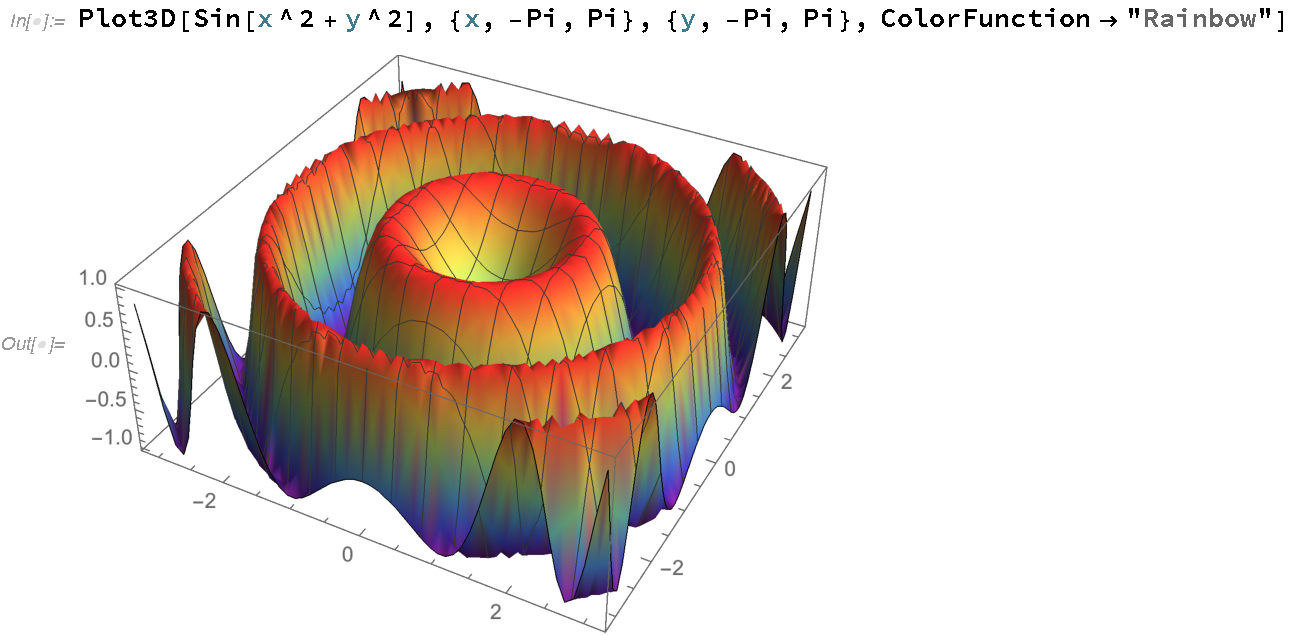
\includegraphics[width=3in]{3Dgraph}

\bigskip

 
\subsection{Using figures}

In most cases, you want to put a graphic inside of 
a \texttt{figure} environment, which handles
captions, numbering, spacing and placement. 
In the source file, there is a figure specified right \textbf{here}...
 \begin{figure}
 \centering
 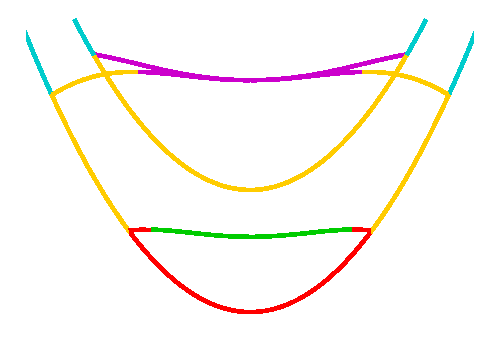
\includegraphics[width=2 in]{perfect_diagram}
\caption{A pretty bifurcation diagram}
 \label{perfect_fig}
 \end{figure}
 However, as you can see, Figure~\ref{perfect_fig} is not quite here in the output file. Instead, \LaTeX\ chooses where
 to place the figure, based on
available space. In this case, Figure\ \ref{perfect_fig}  is at the top of the page. The placement of figures can be adjusted--- there is good documentation
in \href{http://en.wikibooks.org/wiki/LaTeX/Floats,_Figures_and_Captions}{Floats and Figures}  section of the LaTeX Wikibook \cite{wikibook}.
Note: it is good style for all figures to be referenced directly in the text.

\section{Citations and Bibliographies}


This section shows you how to create your bibliography and citations using two tools: an auxiliary program called BibTeX, and the LaTeX package called biblatex. 
The main advantages of BibTeX/biblatex are
\begin{enumerate}
\item the software handles the formatting of the bibliography entries,
\item you can import bibliographic information straight from the web.
\end{enumerate}
Here, I present basic information only; for more, see, for example, the section called 
\href{https://en.wikibooks.org/wiki/LaTeX/Bibliography_Management}{``Bibliography Management"} in the LaTeX Wikibook \cite[\S 5.3]{wikibook}.

\subsection{Finding bibliographic data}

Several online research tools allow you to export bibliographic information in the BibTeX format. Below are detailed instructions for MathSciNet and Google Scholar.

\begin{description}
\item[MathSciNet]
On the review page for your source, there is a drop-down menu labeled ``Select alternative format". Choose ``BibTeX". 
\item[Google Scholar]
Search for your source. Below the search result, click on the ``Cite" link. Then click on ``BibTeX" at the bottom of the window. 
\end{description}
In both cases above, your browser window contains a bibliographic record in BibTeX format. Select the record with your mouse and copy it so that you can to paste it into your bibliographic database--- see the next section.

Besides online search tools, some bibliography management software  can export data in BibTeX format. Using both online search tools and bibliography software, you might never need to type bibliographic information by hand; however, if you do need to, then you can simply duplicate an existing entry and modify it. For the finer points of how to create a \href{https://en.wikibooks.org/wiki/LaTeX/Bibliography_Management}{BibTeX record}, see \cite[\S 5.3.3.1--5]{wikibook}.

\subsection{Making a bibliographic database}
A BibTeX database file is a plain text file. For example, the database file that accompanies this document is called \texttt{sample.bib}; you can open it with any text editor (e.g.\ TeXShop or TexWorks, or the built-in editors TextEdit on a Mac and Notepad on a Windows computer) and poke around. When you are creating your own BibTeX database, the easiest thing to do is delete all of the text in \texttt{sample.bib}, paste in your bibliographic entries, then rename the file. Use a filename without spaces and with the extension \texttt{.bib}.\footnote{Spaces in the filename are probably OK on most modern \TeX\ systems, but sometimes can cause  problems.} Save your database file in the same folder as your \LaTeX\ document. For example, if you want to typeset the file that generates this document (\verb+Math399S2019_ThesisTemplate.tex+), then you should put \texttt{sample.bib} in the same folder as this file; see further instructions in Section~\ref{workflow}.

After pasting the bibliographic data in from the web, you may want to tweak the information in your database file, in which case you can simply edit the text file---  but be careful to preserve the punctuation that delineates the records.\footnote{The BibDesk application is free software for Macs that is used for creating, editing and managing BibTeX database files.}
 The most common change to your \texttt{.bib} file is to change the ``citation keys''.  The first entry in each record is its citation key, which is how you refer to the record in your \LaTeX\ source when you make a citation using the \verb+\cite+ command (see Section~\ref{cite} below). MathSciNet uses the MR review number as the citation key, but you will almost certainly  prefer an easier to remember key, like the author's/authors' initials. 

\subsection{Setting up biblatex in your \texttt{.tex} file}
The following two lines already appear in the preamble of this template file:

\smallskip
\begin{verbatim}
\usepackage[backend=bibtex]{biblatex}
\addbibresource{sample.bib}
\end{verbatim}
\smallskip
Replace \texttt{sample.bib} with the name of your database file.

The following line appears at the end of this template (right before the \verb+\end{document}+); this command actually generates the reference list.
\smallskip
\begin{verbatim}
\printbibliography
\end{verbatim}


\subsection{Making citations}  \label{cite}
In the \LaTeX\ source for the text above, you can see some examples of how to use the \verb+\cite+ command to generate citations to items that are in the database file. 
Here are some further examples.

\begin{enumerate}
\item A very interesting but completely unrelated reference is \cite[p.~12]{Di1988}.
\item Compare our main result with that of Diaconis and Graham \cite[Theorem~1]{DiGr1985}.
\end{enumerate}

\subsubsection{Non-cited sources} By default only \emph{cited} sources appear in the reference list that is generated by biblatex. If you have a source that you want to appear in the bibliography, but you don't want to cite it explicitly, then you can use the \verb+\nocite+ command. For example, I have not used the \verb+\cite+ command to cite the paper of Chihara, but it does appear in the bibliography because I have included a corresponding \verb+\nocite+ command in the \LaTeX\ source (right after this text). 
\nocite{MR871831}  % \nocite command here to force the paper to appear in the reference list
(On the other hand, a paper by Allendoerfer appears in \texttt{sample.bib}, but does not appear in the reference list of this paper, since there is no corresponding \verb+\cite+ command and no corresponding \verb+\nocite+ command.)

\subsection{Workflow}\label{workflow}

Generating a pdf with references and citations takes a surprising number of steps--- but each step is only a click followed by a short wait. I illustrate the steps below for this file, \verb+Math399S2019_ThesisTemplate.tex+. (The footnotes tell you roughly what is happening at each step, but you don't need that information to get started.)

\begin{enumerate} 
\item First, run \LaTeX\ on \verb+Math399S2019_ThesisTemplate.tex+, as usual--- you do this  by simply pressing the ``Go" button in your front-end program.\footnote{This step not only 
produces \texttt{.pdf} file that you are familiar with, but also generates an \texttt{.aux} file which contains (among other things) the name of the BibTeX database file (as specified in the \texttt{addbibreseource} command) and the list of citations made via the \texttt{cite} command. This \texttt{.aux} file is needed in the next step. At this stage, the citations in the pdf are marked as [?], since the bibliography has not been built yet.}
\item Run BibTeX on \verb+Math399S2019_ThesisTemplate.tex+; to do so, click on the drop-down menu next to the ``Go" button, choose the ``BibTeX" action, and then click ``Go".\footnote
{In this step, BibTeX scans both the \texttt{.aux} file from the previous step and the database file. It finds all the items in the database that are referenced by 
\texttt{cite} commands and builds the bibliography accordingly, storing it in a \texttt{.bbl} file. No changes are made to the pdf.}
\item Re-run \LaTeX\ on \verb+Math399S2019_ThesisTemplate.tex+: switch the drop-down menu back to ``LaTeX"/``pdfLaTeX" and click ``Go".\footnote{Here, the biblatex package typesets the reference list, adding it to the pdf output. Some citations may still be marked as [?], to be adjusted in the next step.}
\item Finally, run  \LaTeX\ on \verb+Math399S2019_ThesisTemplate.tex+ one more time.\footnote{In this last step, \LaTeX\ inserts correct citation numbers.}
\end{enumerate} 

That's it! The process is only a bit more complicated than typesetting a vanilla \LaTeX\ document. If you run into trouble, the warnings and errors that appear in the console window may help you straighten things out.\footnote{If you run into untraceable errors, it can sometimes help to delete the \texttt{.aux} and \texttt{.bbl} files and start afresh.} %In TeXShop, choose the menu item \texttt{File->Trash Aux Files}.}


\newpage
\section*{Acknowledgments} % OPTIONAL: non-numbered section for acknowledgements

This template is descended from a long line of sample files that have been circulated in the department over the years, not only the publicly available documents \cite{cg} and \cite{em}, but also other internal documents created by Rob Manning, Josh Sabloff and David Lippel. (Note: in the thesis, an acknowledgements section is optional; one is included here to show you the appropriate typesetting commands.)

\bigskip
This is a random reference.\cite{hello}

\bigskip


%%-------------------------------------------------------------------------------------------------
%% CUT STOP: preserve the command below to generate the reference list

\printbibliography

\end{document}

